\documentclass[conference]{IEEEtran}
\IEEEoverridecommandlockouts

% =====================================================
% PACKAGES
% =====================================================

\usepackage{cite}
\usepackage{amsmath,amssymb,amsfonts}
\usepackage{graphicx}
\usepackage{textcomp}
\usepackage{xcolor}
\usepackage{booktabs}
\usepackage{multirow}
\usepackage{array}
\usepackage{float}

% =====================================================
% DOCUMENT
% =====================================================

\begin{document}

% =====================================================
% TITLE
% =====================================================

\title{
Comparative Analysis of Normalization and Cross-Validation Scenarios for Deep Learning-Based Dengue Fever Classification
}

% =====================================================
% AUTHOR
% =====================================================

\author{

\IEEEauthorblockN{Ramadhani Vanva Fauzia}
\IEEEauthorblockA{
\textit{Information Systems Department} \\
\textit{Telkom University Surabaya} \\
Surabaya, Indonesia \\
Ramadhanivanva@student.telkomuniversity.ac.id
}

}

% =====================================================
% TITLE AREA
% =====================================================

\maketitle

% =====================================================
% ABSTRACT
% =====================================================

\begin{abstract}

% Fill abstract here

\end{abstract}

% =====================================================
% KEYWORDS
% =====================================================

\begin{IEEEkeywords}
Deep Learning, Dengue Fever, Artificial Neural Network, Classification, Normalization, Cross Validation
\end{IEEEkeywords}

% =====================================================
% INTRODUCTION
% =====================================================

\section{Introduction}

Dengue Fever is one of the most significant mosquito-borne infectious diseases in tropical and subtropical countries. According to the \textit{World Health Organization (WHO)}, the global incidence of Dengue has increased rapidly over the past decades, particularly in Southeast Asia and other tropical regions. Early detection and classification of Dengue Fever are essential to reduce mortality rates and improve clinical treatment effectiveness \cite{b1}.

Conventional diagnosis of Dengue Fever generally relies on clinical symptoms and laboratory examinations performed by healthcare professionals. Common symptoms include fever, headache, nausea, muscle pain, and skin rash, while laboratory indicators such as platelet count, hematocrit, leukocyte count, and hemoglobin level are often used to support diagnosis. However, manual interpretation of clinical data may require considerable time and may be affected by human error, especially when the number of patients increases significantly \cite{b2}.

Recent developments in Artificial Intelligence (AI) and Deep Learning have demonstrated promising performance in medical classification and prediction systems. Deep Learning models are capable of learning complex non-linear relationships from medical datasets and have been widely applied in disease diagnosis, image classification, and healthcare decision support systems \cite{b3}. Among various Deep Learning approaches, Artificial Neural Network (ANN) models have shown good capability in binary classification problems due to their ability to capture hidden patterns within clinical datasets \cite{b4}.

Several previous studies have implemented Machine Learning and Deep Learning techniques for Dengue prediction and classification. However, many studies mainly focus on model performance without comprehensively analyzing the influence of preprocessing techniques such as data normalization and validation strategies. In fact, normalization techniques can significantly affect Deep Learning performance because numerical feature scales may influence the convergence process during model training \cite{b5}. Furthermore, Cross Validation is important to evaluate model stability and generalization capability in healthcare datasets \cite{b6}.

Therefore, this study proposes a Deep Learning-based Dengue Fever classification system using clinical symptom and laboratory examination datasets. This research focuses on comparative analysis of normalization techniques and Cross Validation scenarios to determine the optimal classification performance. Two dataset scenarios were evaluated, including a full dataset consisting of symptom and laboratory features, and a symptom-only dataset. Three normalization methods were implemented, namely without normalization, StandardScaler, and MinMaxScaler, resulting in six experimental scenarios. In addition, K-Fold Cross Validation was applied to evaluate the robustness and stability of the proposed model.

The results of this study are expected to contribute to the development of healthcare decision support systems and provide insights regarding the influence of preprocessing techniques on Deep Learning-based medical classification systems.

\subsection{Research Contributions}

The main contributions of this study are summarized as follows:

\begin{itemize}

\item Comparative analysis of normalization techniques for Dengue Fever classification.

\item Comparative analysis between full dataset and symptom-only dataset.

\item Evaluation of model stability using K-Fold Cross Validation.

\item Development of a Deep Learning-based healthcare classification system.

\item Investigation of the influence of clinical symptoms and laboratory examination features on classification performance.

\item Evaluation of the effectiveness of StandardScaler and MinMaxScaler normalization techniques in improving Deep Learning performance.

\item Analysis of model generalization capability through multiple cross-validation scenarios.

\item Identification of the best experimental scenario based on classification performance metrics including Accuracy, Precision, Recall, F1-Score, and ROC-AUC.

\item Development of an experimental framework that can be applied to other healthcare classification problems using Deep Learning approaches.

\end{itemize}

% =====================================================
% RELATED WORK
% =====================================================

\section{Related Work}

\begin{table}[H]
\caption{Summary of Related Studies}
\centering
\begin{tabular}{|c|c|c|}
\hline
\textbf{Study} & \textbf{Method} & \textbf{Accuracy} \\
\hline
Study A & ANN & 92\% \\
\hline
Study B & CNN & 94\% \\
\hline
Study C & Random Forest & 89\% \\
\hline
\end{tabular}
\label{tab_related}
\end{table}

% =====================================================
% RESEARCH METHODOLOGY
% =====================================================

\section{Research Methodology}

% =====================================================
% WORKFLOW
% =====================================================

\subsection{Research Workflow}

\begin{figure}[H]
\centering
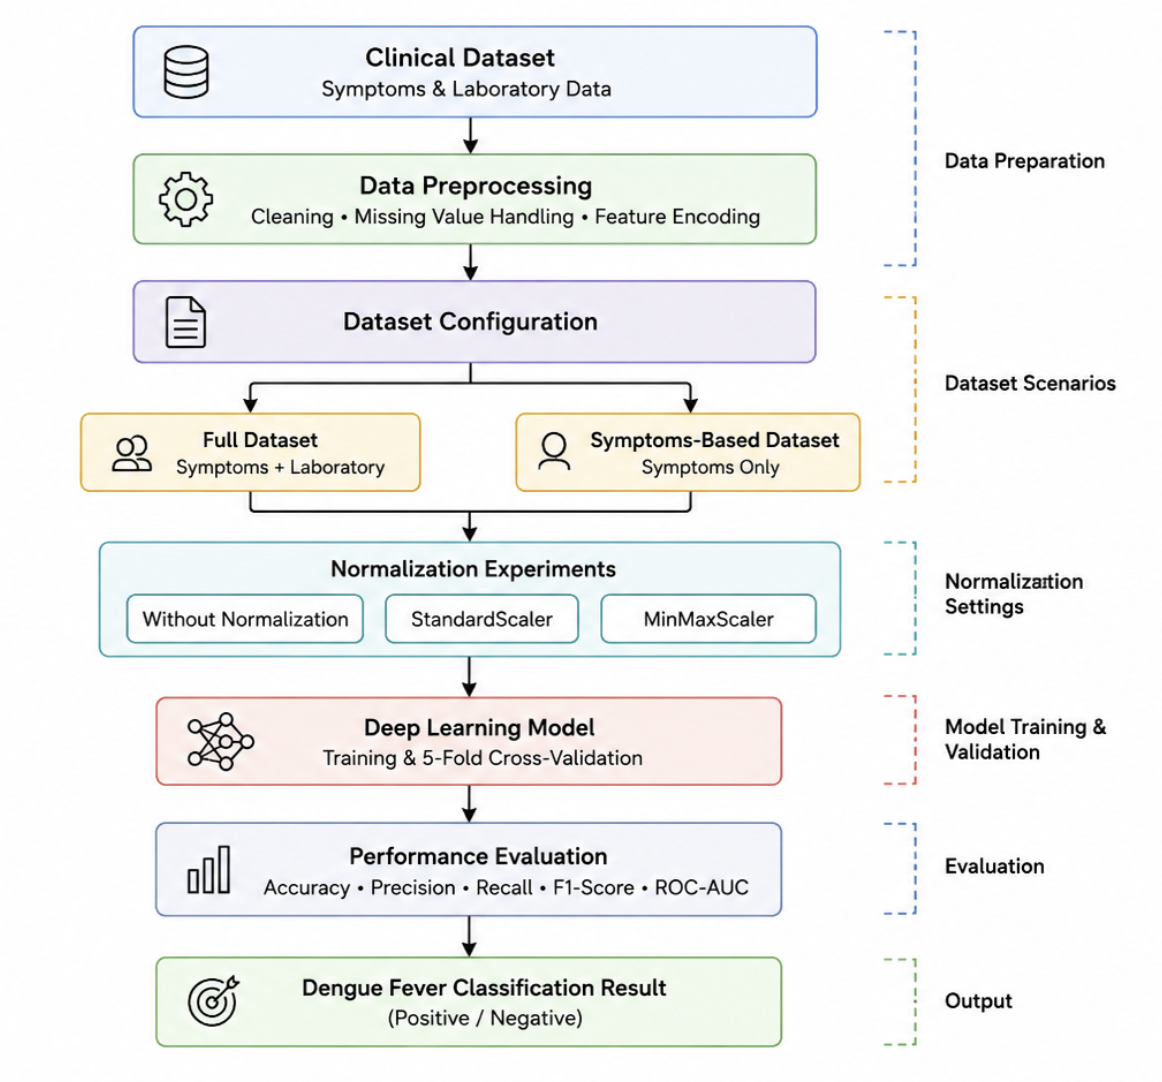
\includegraphics[width=0.48\textwidth]{workflow.png}
\caption{Research Workflow}
\label{fig_workflow}
\end{figure}

% =====================================================
% DATASET
% =====================================================

\subsection{Dataset}

The dataset used in this study consists of clinical symptom and laboratory examination data.

\begin{table}[H]
\caption{Dataset Attribute Categories}
\centering
\begin{tabular}{|c|c|}
\hline
\textbf{Category} & \textbf{Number of Features} \\
\hline
Symptoms & 9 \\
\hline
Laboratory Features & 4 \\
\hline
Total Features & 13 \\
\hline
\end{tabular}
\label{tab_dataset}
\end{table}

% =====================================================
% DATASET SCENARIO
% =====================================================

\subsection{Dataset Scenarios}

Two dataset scenarios were evaluated in this study.

\begin{table}[H]
\caption{Dataset Scenarios}
\centering
\begin{tabular}{|c|m{5cm}|}
\hline
\textbf{Scenario} & \textbf{Dataset Composition} \\
\hline
Scenario 1 & Symptoms + Laboratory Features \\
\hline
Scenario 2 & Symptoms Features Only \\
\hline
\end{tabular}
\label{tab_scenario}
\end{table}

% =====================================================
% PREPROCESSING
% =====================================================

\subsection{Data Preprocessing}

The preprocessing stage includes:

\begin{itemize}

\item Data Cleaning

\item Missing Value Handling

\item Feature Encoding

\item Data Normalization

\end{itemize}

% =====================================================
% NORMALIZATION
% =====================================================

\subsection{Normalization Experiments}

Three normalization methods were evaluated:

\begin{itemize}

\item Without Normalization

\item StandardScaler

\item MinMaxScaler

\end{itemize}

\begin{table}[H]
\caption{Normalization Experiment Scenarios}
\centering
\begin{tabular}{|c|c|c|}
\hline
\textbf{Experiment} & \textbf{Dataset} & \textbf{Normalization} \\
\hline
Exp-1 & Full Dataset & None \\
\hline
Exp-2 & Full Dataset & StandardScaler \\
\hline
Exp-3 & Full Dataset & MinMaxScaler \\
\hline
Exp-4 & Symptoms Only & None \\
\hline
Exp-5 & Symptoms Only & StandardScaler \\
\hline
Exp-6 & Symptoms Only & MinMaxScaler \\
\hline
\end{tabular}
\label{tab_norm}
\end{table}

% =====================================================
% DEEP LEARNING MODEL
% =====================================================

\subsection{Proposed Deep Learning Model}

\begin{table}[H]
\caption{ANN Architecture}
\centering
\begin{tabular}{|c|c|c|}
\hline
\textbf{Layer} & \textbf{Neurons} & \textbf{Activation} \\
\hline
Input Layer & 13 & - \\
\hline
Dense Layer 1 & 64 & ReLU \\
\hline
Dropout Layer & - & - \\
\hline
Dense Layer 2 & 32 & ReLU \\
\hline
Output Layer & 1 & Sigmoid \\
\hline
\end{tabular}
\label{tab_model}
\end{table}

\begin{figure}[H]
\centering
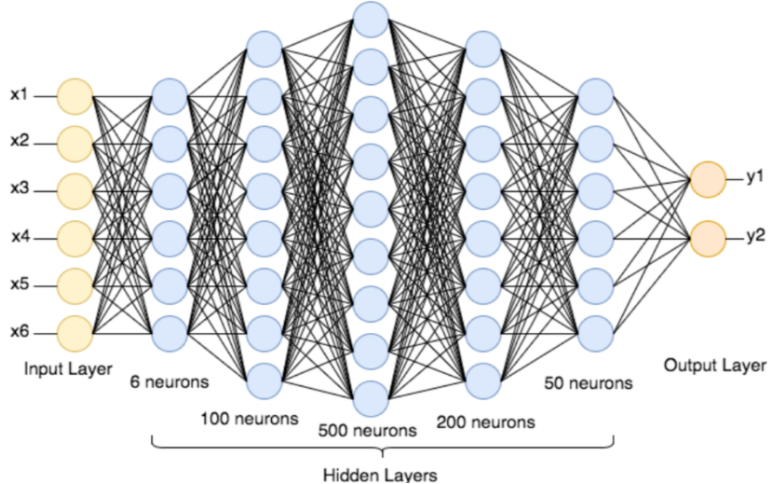
\includegraphics[width=0.47\textwidth]{deeplearning_architecture.png}
\caption{Artificial Neural Network Architecture}
\label{fig_ann}
\end{figure}

% =====================================================
% CROSS VALIDATION
% =====================================================

\subsection{Cross Validation}

K-Fold Cross Validation with K=5 was implemented to evaluate model stability and generalization capability.

\begin{table}[H]
\caption{Cross Validation Scenarios}
\centering
\begin{tabular}{|c|c|c|}
\hline
\textbf{Scenario} & \textbf{Dataset} & \textbf{Normalization} \\
\hline
CV-1 & Full Dataset & None \\
\hline
CV-2 & Full Dataset & StandardScaler \\
\hline
CV-3 & Full Dataset & MinMaxScaler \\
\hline
CV-4 & Symptoms Only & None \\
\hline
CV-5 & Symptoms Only & StandardScaler \\
\hline
CV-6 & Symptoms Only & MinMaxScaler \\
\hline
\end{tabular}
\label{tab_cv_scenario}
\end{table}

% =====================================================
% EVALUATION METRICS
% =====================================================

\subsection{Evaluation Metrics}

The evaluation metrics used in this study include:

\begin{itemize}

\item Accuracy

\item Precision

\item Recall

\item F1-Score

\item ROC-AUC

\end{itemize}

% =====================================================
% RESULTS AND DISCUSSION
% =====================================================

\section{Results and Discussion}

% =====================================================
% TRAINING PERFORMANCE
% =====================================================

\subsection{Training Performance}

\begin{figure}[H]
\centering
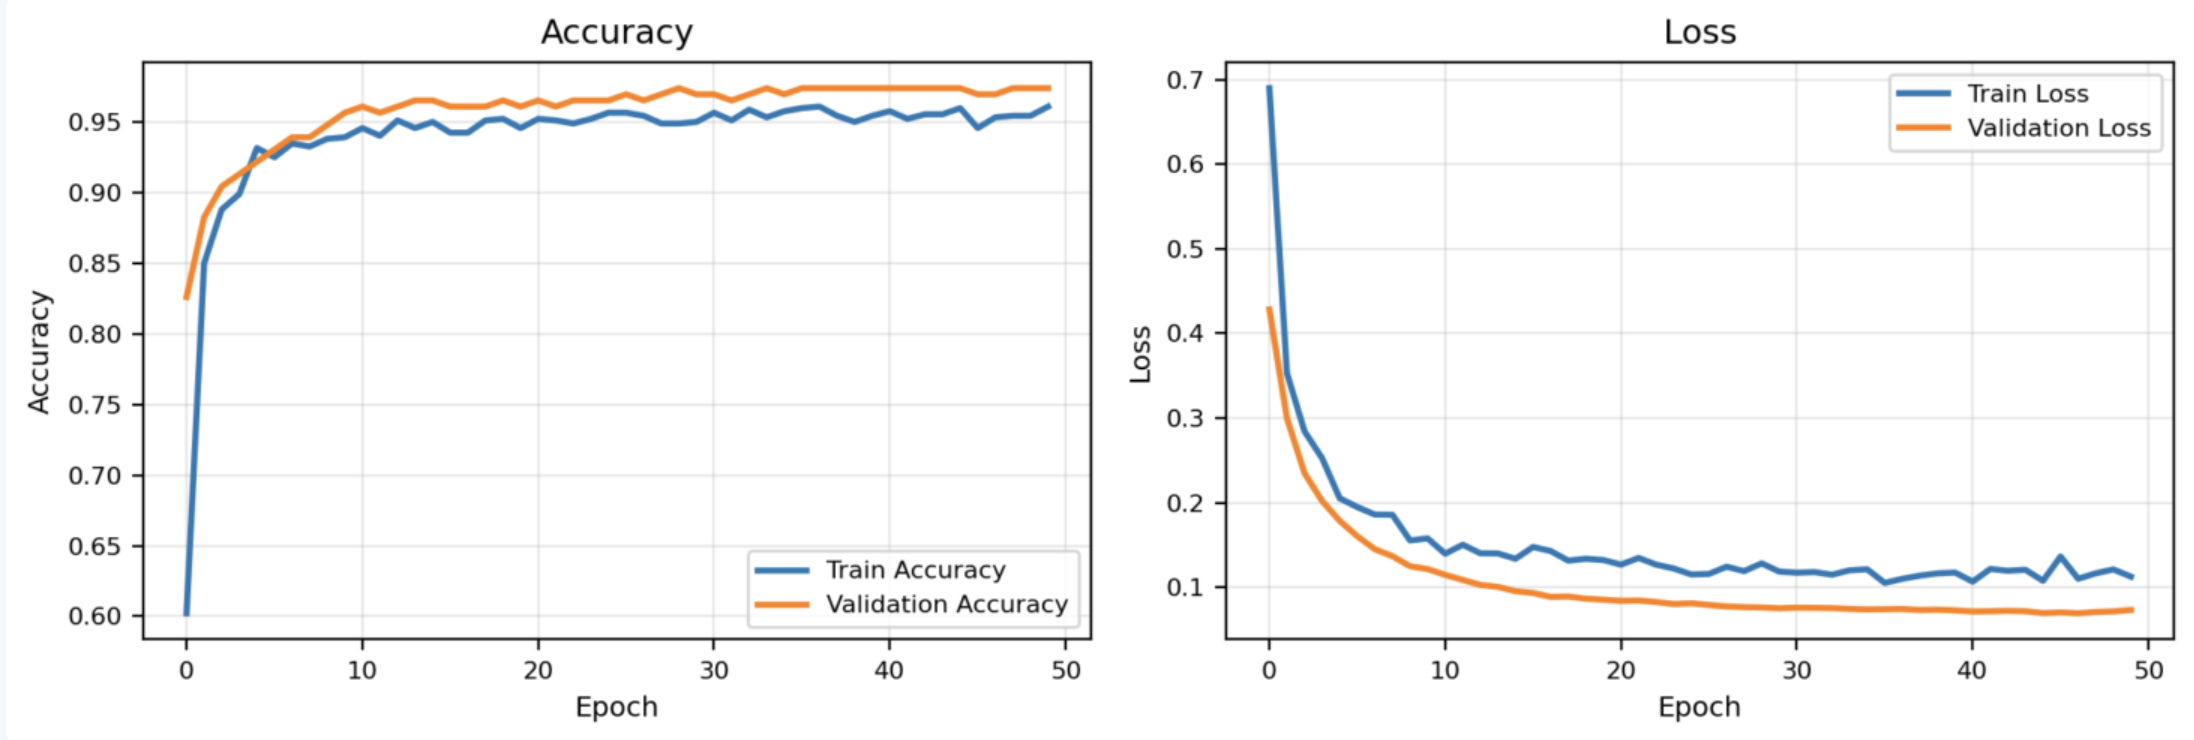
\includegraphics[width=0.48\textwidth]{training acc&loss.png}
\caption{Training Accuracy and Loss}
\label{fig_training}
\end{figure}

% Discussion about convergence and model learning

% =====================================================
% NORMALIZATION RESULT
% =====================================================

\subsection{Normalization Experiment Results}

\begin{table}[H]
\caption{Experimental Results}
\centering
\begin{tabular}{|c|c|c|c|c|}
\hline
\textbf{Experiment} & \textbf{Accuracy} & \textbf{Precision} & \textbf{Recall} & \textbf{F1-Score} \\
\hline
Exp-1 &  &  &  &  \\
\hline
Exp-2 &  &  &  &  \\
\hline
Exp-3 &  &  &  &  \\
\hline
Exp-4 &  &  &  &  \\
\hline
Exp-5 &  &  &  &  \\
\hline
Exp-6 &  &  &  &  \\
\hline
\end{tabular}
\label{tab_experiment}
\end{table}

\begin{figure}[H]
\centering
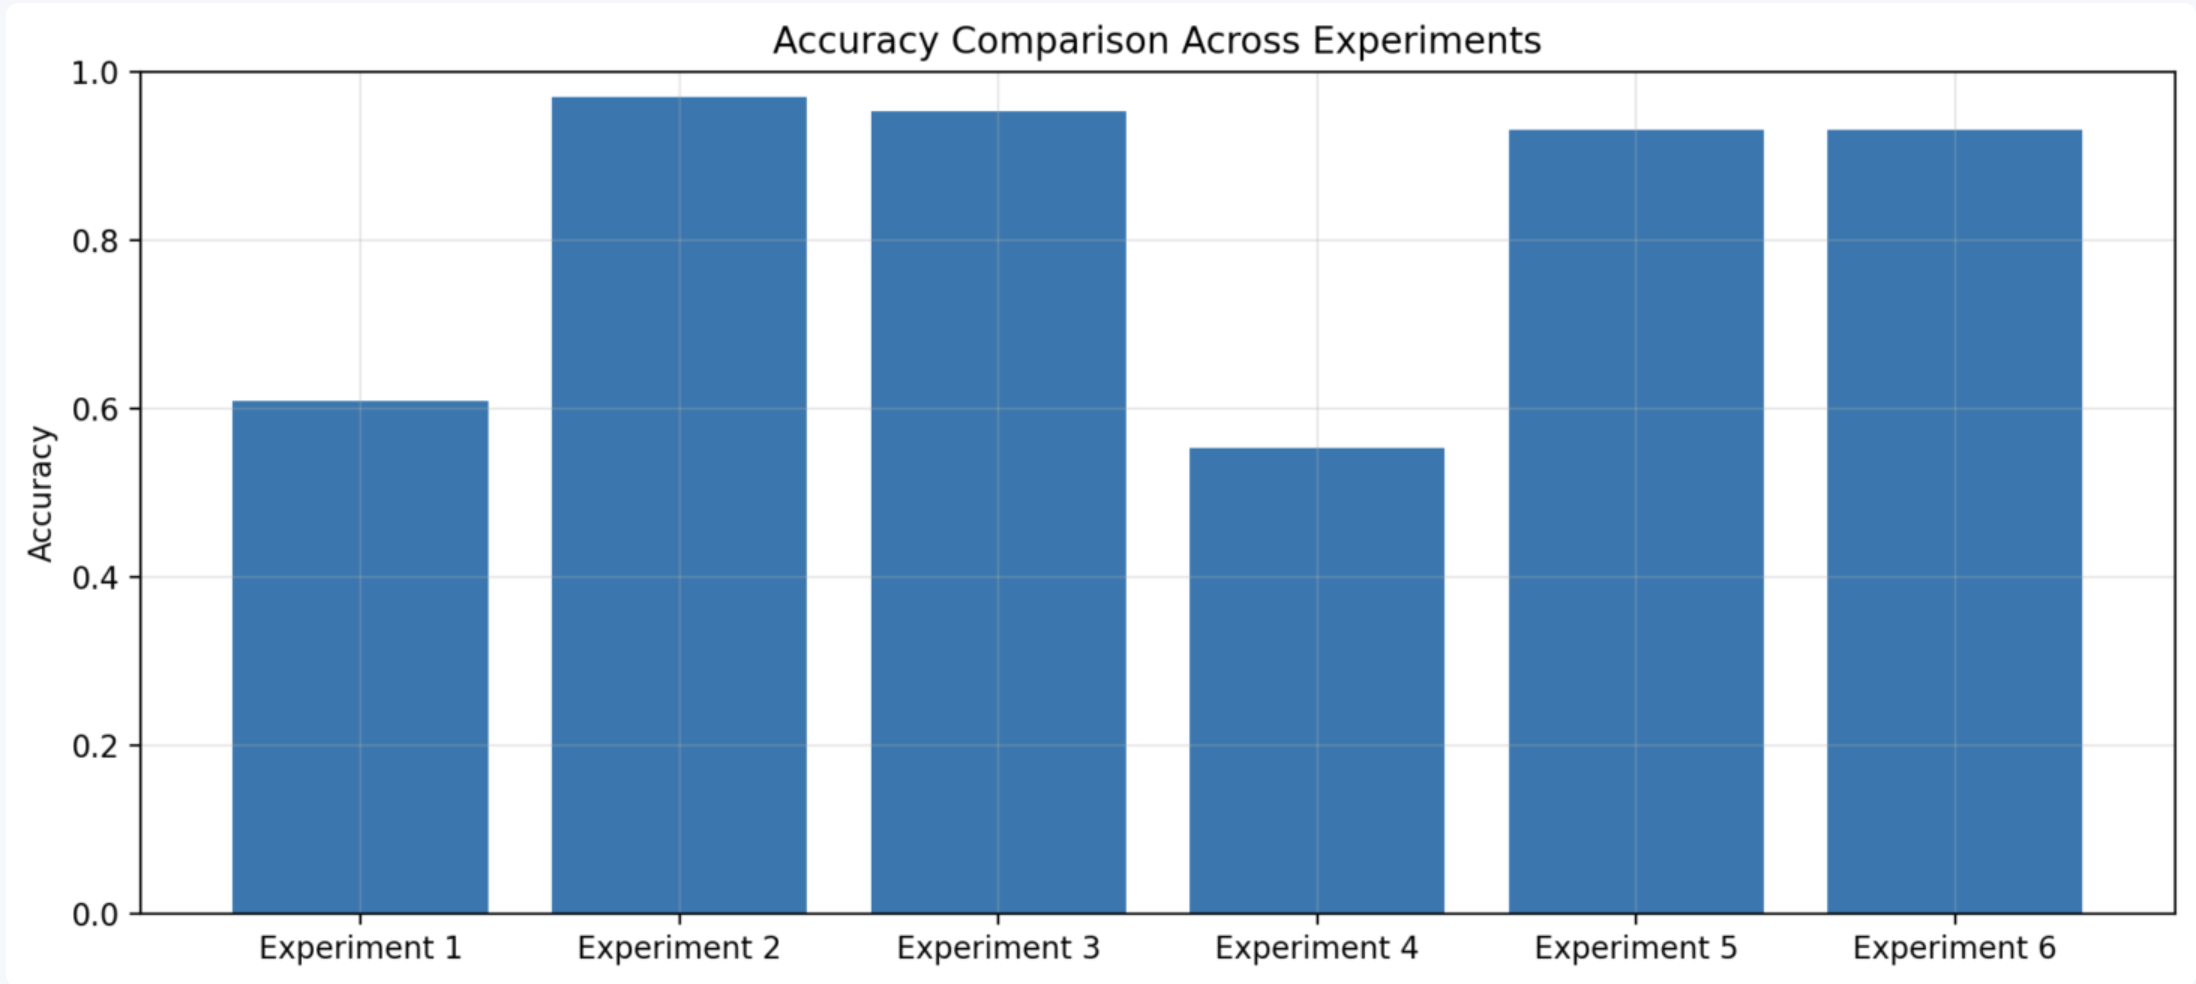
\includegraphics[width=0.48\textwidth]{normalization_comparison.png}
\caption{Comparison of Experimental Accuracy}
\label{fig_experiment}
\end{figure}

% =====================================================
% CROSS VALIDATION RESULT
% =====================================================

\subsection{Cross Validation Results}

\begin{table}[H]
\caption{Cross Validation Results}
\centering
\begin{tabular}{|c|c|c|}
\hline
\textbf{Scenario} & \textbf{Mean Accuracy} & \textbf{Std Deviation} \\
\hline
CV-1 &  &  \\
\hline
CV-2 &  &  \\
\hline
CV-3 &  &  \\
\hline
CV-4 &  &  \\
\hline
CV-5 &  &  \\
\hline
CV-6 &  &  \\
\hline
\end{tabular}
\label{tab_cv_result}
\end{table}

\begin{figure}[H]
\centering
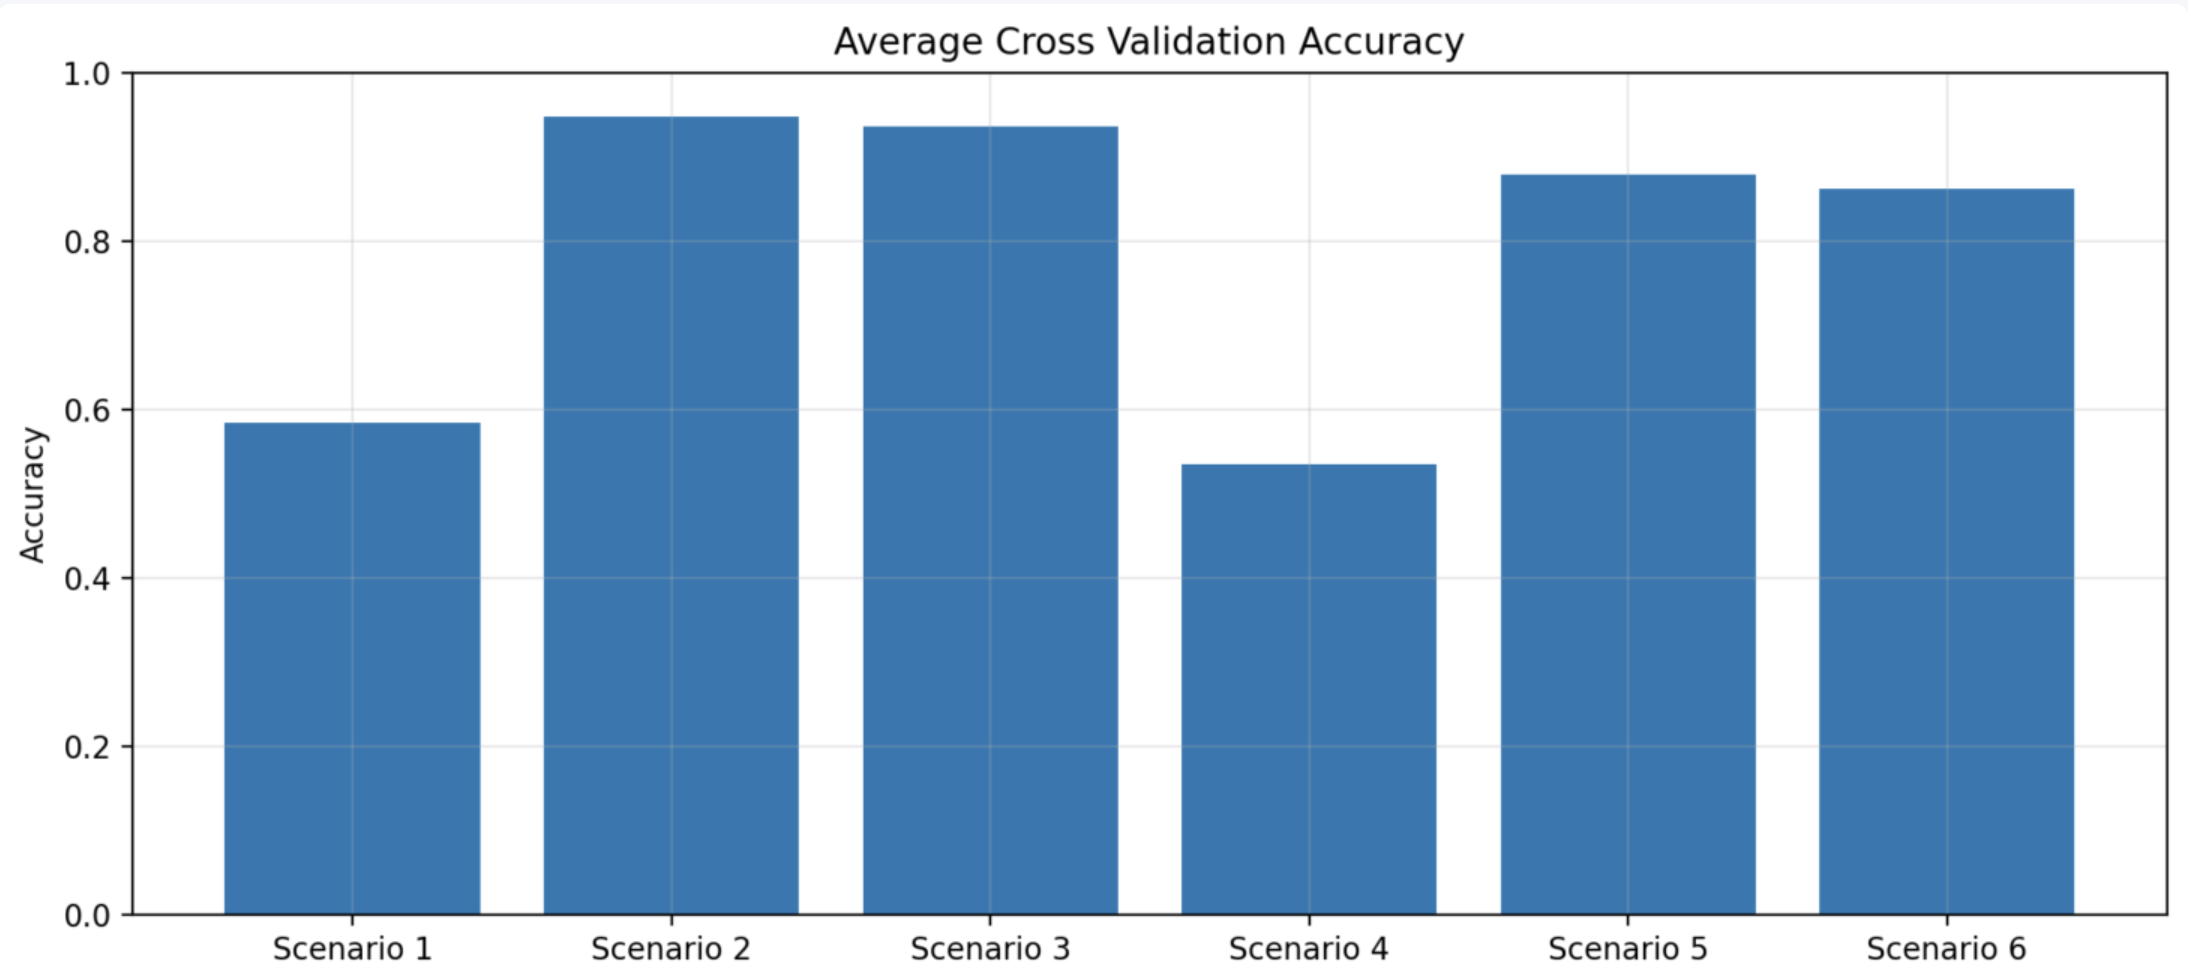
\includegraphics[width=0.48\textwidth]{cv_comparison.png}
\caption{Cross Validation Accuracy Comparison}
\label{fig_cv}
\end{figure}

% =====================================================
% CONFUSION MATRIX
% =====================================================

\subsection{Confusion Matrix Analysis}

\begin{figure}[H]
\centering
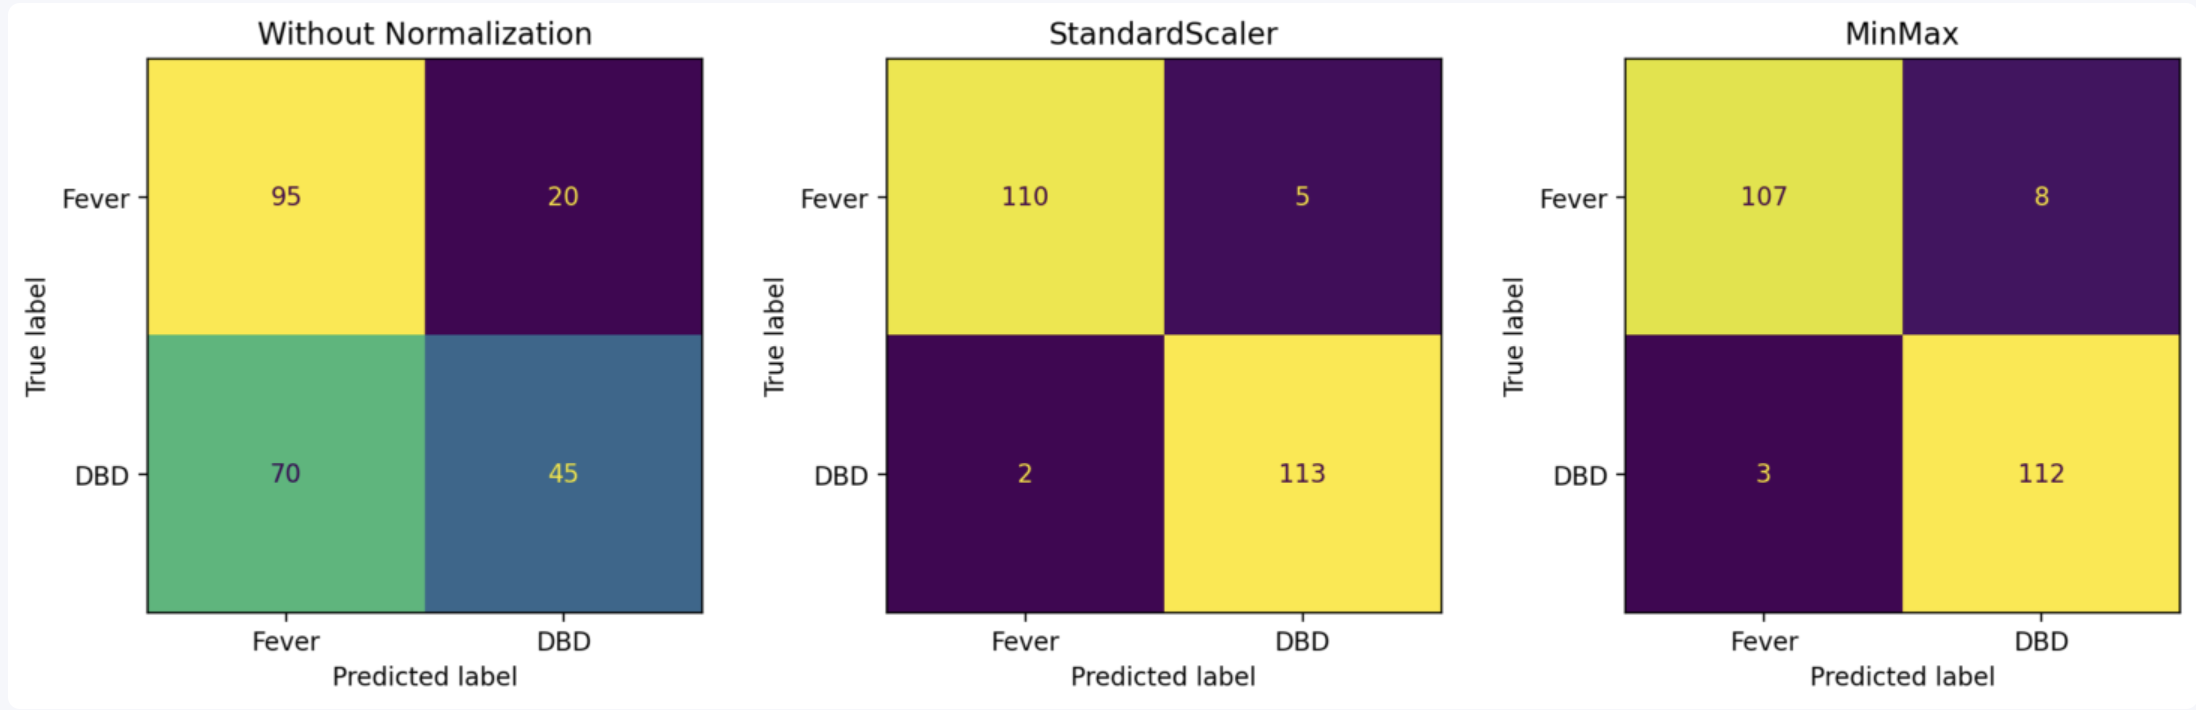
\includegraphics[width=0.48\textwidth]{confusion_matrix.png}
\caption{Confusion Matrix Comparison for Three Normalization Methods}
\label{fig_cm}
\end{figure}

% =====================================================
% ROC CURVE
% =====================================================

\subsection{ROC Curve Analysis}

\begin{figure}[H]
\centering
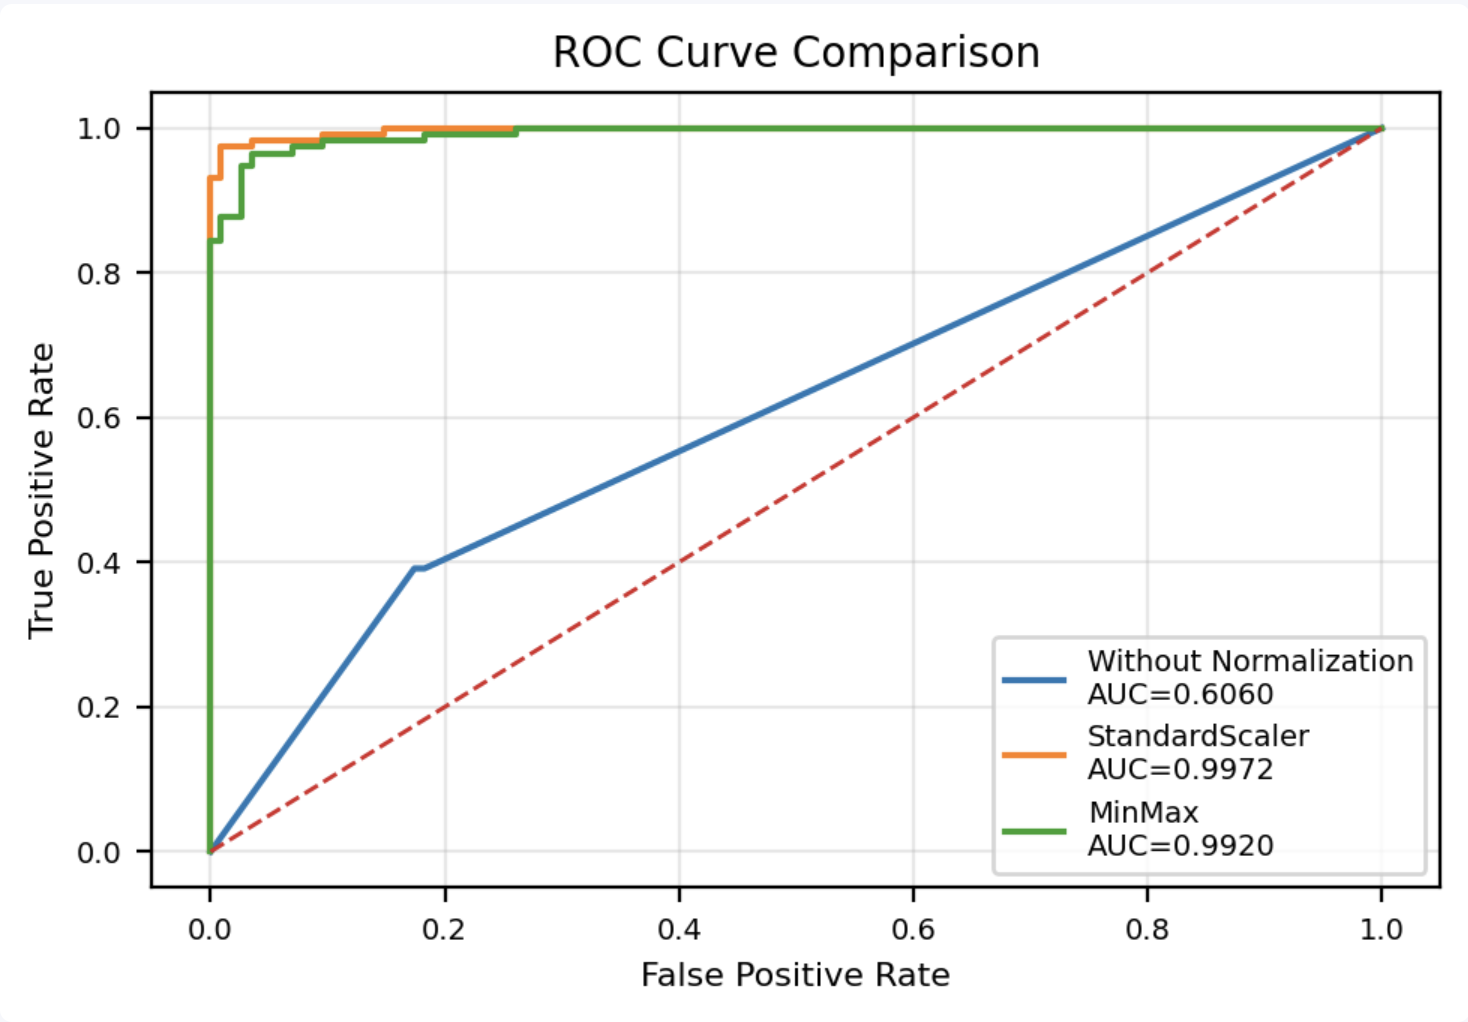
\includegraphics[width=0.48\textwidth]{ROC.png}
\caption{ROC Curve Comparison for Three Normalization Methods}
\label{fig_roc}
\end{figure}

% =====================================================
% DISCUSSION
% =====================================================

\subsection{Discussion}

% Discussion about:
% - Best normalization
% - Effect of laboratory features
% - Model stability
% - Performance comparison
% - Healthcare implementation

% =====================================================
% CONCLUSION
% =====================================================

\section{Conclusion}

% Fill conclusion here

% =====================================================
% FUTURE WORK
% =====================================================

\section{Future Work}

% Fill future work here

% =====================================================
% ACKNOWLEDGMENT
% =====================================================

\section*{Acknowledgment}

% Optional acknowledgment

% =====================================================
% REFERENCES
% =====================================================

\begin{thebibliography}{00}

\bibitem{b1}
World Health Organization, 
``Dengue and Severe Dengue,'' 
WHO Fact Sheets, 2024. 
[Online]. Available: https://www.who.int/news-room/fact-sheets/detail/dengue-and-severe-dengue

\bibitem{b2}
S. Simmons, J. Farrar, N. van Vinh Chau, and B. Wills,
``Dengue,'' 
\textit{New England Journal of Medicine}, 
vol. 366, no. 15, pp. 1423--1432, 2012.

\bibitem{b3}
Y. LeCun, Y. Bengio, and G. Hinton,
``Deep Learning,'' 
\textit{Nature}, 
vol. 521, no. 7553, pp. 436--444, 2015.

\bibitem{b4}
I. Goodfellow, Y. Bengio, and A. Courville,
\textit{Deep Learning}. 
Cambridge, MA, USA: MIT Press, 2016.

\bibitem{b5}
S. Raschka and V. Mirjalili,
\textit{Python Machine Learning: Machine Learning and Deep Learning with Python, scikit-learn, and TensorFlow}. 
3rd ed. Birmingham, U.K.: Packt Publishing, 2019.

\bibitem{b6}
T. Hastie, R. Tibshirani, and J. Friedman,
\textit{The Elements of Statistical Learning}. 
2nd ed. New York, NY, USA: Springer, 2009.

\end{thebibliography}


% =====================================================
% END DOCUMENT
% =====================================================

\end{document}